%!TEX TS-program = xelatex

\documentclass[a4paper,12pt, landscape]{article}

\usepackage[english,russian]{babel}   %% загружает пакет многоязыковой вёрстки
\usepackage{fontspec}      %% подготавливает загрузку шрифтов Open Type, True Type и др.
\defaultfontfeatures{Ligatures={TeX},Renderer=Basic}  %% свойства шрифтов по умолчанию
\setmainfont[Ligatures={TeX,Historic},
SmallCapsFont={Brill},
SmallCapsFeatures={Letters=SmallCaps}]{Brill} %% задаёт основной шрифт документа
\setsansfont{Brill}                    %% задаёт шрифт без засечек
\setmonofont{Noto Sans Ethiopic}
\usepackage{indentfirst}

%%% Дополнительная работа с математикой
\usepackage{amsmath,amsfonts,amssymb,amsthm,mathtools} % AMS
\usepackage{icomma} % "Умная" запятая: $0,2$ --- число, $0, 2$ --- перечисление

%%% Работа с картинками
\usepackage{wrapfig} % Обтекание рисунков текстом
\usepackage{subcaption}
\usepackage{rotating}
\usepackage{fixltx2e}
\usepackage{hhline}
\usepackage{lscape}
\usepackage[usenames,dvipsnames,svgnames,table,rgb]{xcolor}%пакет для использования цветов 

\usepackage{enumitem}
\setlist{nolistsep, leftmargin=5mm}

%%% Работа с таблицами
\usepackage{array,tabularx,tabulary,booktabs} % Дополнительная работа с таблицами
\usepackage{longtable}  % Длинные таблицы
\usepackage{multirow} % Слияние строк в таблице

\usepackage{multicol} % Несколько колонок

%%% Страница
\usepackage{extsizes} % Возможность сделать 14-й шрифт
\usepackage[twocolumn]{geometry} % Простой способ задавать поля
	\geometry{top=12mm}
	\geometry{bottom=13mm}
	\geometry{left=13mm}
	\geometry{right=9mm}

%\usepackage{fancyhdr} % Колонтитулы
% 	\pagestyle{fancy}
 	%\renewcommand{\headrulewidth}{0pt}  % Толщина линейки, отчеркивающей верхний колонтитул
% 	\lfoot{Нижний левый}
% 	\rfoot{Нижний правый}
% 	\rhead{Верхний правый}
% 	\chead{Верхний в центре}
% 	\lhead{Верхний левый}
%	\cfoot{Нижний в центре} % По умолчанию здесь номер страницы

\usepackage{setspace} % Интерлиньяж
%\onehalfspacing % Интерлиньяж 1.5
%\doublespacing % Интерлиньяж 2
\singlespacing % Интерлиньяж 1

\usepackage{lastpage} % Узнать, сколько всего страниц в документе.
\usepackage{soul} % Модификаторы начертания
\usepackage{bbding}
\usepackage{hyperref}
\usepackage[usenames,dvipsnames,svgnames,table,rgb]{xcolor}
\hypersetup{				% Гиперссылки
    colorlinks=true,       	% false: ссылки в рамках; true: цветные ссылки
    linkcolor=black,          % внутренние ссылки
    citecolor=black,        % на библиографию
    filecolor=black,      % на файлы
    urlcolor=ForestGreen          % на URL
}

\usepackage{environ}
\makeatletter
\newsavebox{\measure@tikzpicture}
\NewEnviron{scaletikzpicturetowidth}[1]{%
	\def\tikz@width{#1}%
	\def\tikzscale{1}\begin{lrbox}{\measure@tikzpicture}%
		\BODY
	\end{lrbox}%
	\pgfmathparse{#1/\wd\measure@tikzpicture}%
	\edef\tikzscale{\pgfmathresult}%
	\BODY
}
\makeatother

\usepackage{pgfplots}
\usepackage{pgfplotstable}
\usepackage{verbatim}

\usepackage{attachfile2}
 \attachfilesetup{appearance=true,
color=0 0 0
 }

%%% Лингвистические пакеты
%\usepackage{savetrees} % пакет, который экономит место
\usepackage{forest} % для рисования деревьев
\usepackage{vowel} % для рисования трапеций гласных
\usepackage{natbib}
\bibpunct[: ]{[}{]}{;}{a}{}{,}
\usepackage[nogroupskip,nopostdot, nonumberlist]{glossaries}
%\usepackage{glossary-mcols} 
%\setglossarystyle{mcolindex}
\usepackage{philex} % пакет для примеров
\addto\captionsrussian{% Replace "english" with the language you use
\renewcommand{\refname}{}
\renewcommand{\glossaryname}{Список глосс}
}
\newcommand{\mytem}{\item[$\circ$]}

\usepackage{todonotes}
\newcounter{mycomment}
\newcommand{\mycom}[1]{
\refstepcounter{mycomment}%
{%
\setstretch{0.7}% spacing
\todo[color=blue!20!white, inline]{%
\textbf{ГМ\themycomment:}~{\footnotesize #1}}%
}}
\renewcommand{\thesection}{\arabic{section}.}
\renewcommand{\thesubsection}{\arabic{section}.\arabic{subsection}}
\setlength{\columnsep}{1.6cm}

\usepackage{sectsty}
\sectionfont{\normalsize}
\subsectionfont{\normalsize}
\usepackage{titlesec}
\titlespacing*{\section}
{0pt}{2ex plus 0ex minus .2ex}{0ex plus .2ex}
\titlespacing*{\subsection}
{0pt}{2ex plus 0ex minus .2ex}{0ex plus .2ex}
\newlength{\bibitemsep}\setlength{\bibitemsep}{.2\baselineskip plus .05\baselineskip minus .05\baselineskip}
\newlength{\bibparskip}\setlength{\bibparskip}{0pt}
\let\oldthebibliography\thebibliography
\renewcommand\thebibliography[1]{%
	\oldthebibliography{#1}%
	\setlength{\parskip}{\bibitemsep}%
	\setlength{\itemsep}{\bibparskip}%
}
\usepackage{alltt}
\begin{document}
\begin{flushright}
	{\footnotesize Г. Мороз, а. Ходзь, Республика Адыгея}
\end{flushright}
\begin{center}{\Large Исследование скорости речи: кубанский диалект\footnote{Автор выражает благодарности:
\begin{itemize}
\mytem Ване Левину, Саше Мартыновой, Лене Пасальской и Соне Сиговой за помощь в придумывании историй;
\mytem Тане Руссите за рисунки;
\mytem информантам ... за неоценимую помощь в проведении исследования;
\mytem ... за комментарии.
\end{itemize}}}
\end{center}
{\noindent\footnotesize последняя версия: \textbf{\href{https://goo.gl/qMgtOd}{https://goo.gl/qMgtOd}}}
\vspace{5mm}
\tableofcontents
\vfill
{~}\\
\pagebreak
\section{Введение}
\subsection{Обзор литературы}
\noindent Судя по всему, о скорости речи говорили еще в начале XX века, но первые квантитативные исследования, начались, видимо, с работ \citep{goldman54} и \citep{goldman56}; и с самых ранних работ данная тема затрагивала еще и некоторые аспекты психиатрии. Данная тема тесно соприкасается с разницей ударных и безударных слогов, а также ритмической структуры слова, фразы и т. п.
\par В исследовании \citep{goldman54} исследовались по три интервью от пяти пациентов, собранных тремя психиатрами. В качестве характеристики скорости речи используется количество слов в минуту и стандартное отклонение полученной величины. В следующей работе \citep{goldman56} автор был более эксплицитен и ввел некоторые важные понятия:
\begin{itemize}
\mytem \textbf{общая скорость речи} (total or overall Speech Rate), которая высчитывается по формуле ${ns}/t$, где ${ns}$ --- это количество слогов во всех высказываниях, a $t$ --- общая длительность всех высказываний.
\mytem \textbf{скорость артикуляции} или \textbf{абсолютная скорость речи} (Articulation Rate), которая высчитывается по формуле $ns/ts$, где $ns$ --- это количество слогов во всех высказываниях, a $ts$ --- время чистого говорения.
\mytem \textbf{пропорциональная длительность пауз}, которая высчитывается по формуле $tp/t$, где $tp$ --- это длительность пауз во всех высказываниях, a $t$ --- общая длительность всех высказываний.
\mytem \textbf{скорость дыхания} (Respiration Rate), которая по формуле $ni/t$, где ${ni}$ --- это количество вдохов во всех высказываниях, a $t$ --- общая длительность всех высказываний.
\end{itemize}
\par Среди результатов работы \citep{goldman56} отмечается отрицательная корреляция между общей скоростью речи и пропорциональной длительностью пауз, т. е. чем длиннее и чем дольше паузы, тем меньше общая скорость речи. В исследовании также подчеркивается, что скорость дыхания, измеряемая в процессе речи, отличается от действительной скорости дыхания, так как в ней происходит выдыхательная задержка, вызванная процессом речепроизводства.
\par Работа \citep{fonagy60} начинается с перечислении идей разных фонетистов о разной скорости, с которой произносятся слова разной длины: длинные слова произносятся быстрее, короткие слова --- медленнее. Потом автор переходит к единицам, которые он называет \textit{ритмическим периодом} (rhythmical period). Автор показывает, что связь между \textbf{средней длиной звука в ритмической единице} экспоненциально зависит от количества звуков в данной единице. В данной работе тоже анализировалось дыхание, а именно информанты читали текст, а исследователь смотрел, где происходит вдох. Длинна ритмической единицы, а следовательно, как считает автор, и скорость, зависят от речевого материала (поэзия, проза, диалог, спортивный комментарий и т. п.), а увеличение скорости в более длинных единицах не связано с дыхательными циклами. 
\par В работе \citep{osser64}  сравнивались скорости речи американских и японских студентов, которая измерялась количеством фонем в минуту. Обнаружилось, что в среднем японские студенты говорили несколько медленнее, однако разница не была статистически значимой. Кроме того, исследователи провели довольно странный эксперимент, в котором они просили респондентов назвать как можно больше слов за одну минуту. Японцы и здесь показали меньший результат, но и в этом эксперименте разница была статистически не значимой. Авторы продолжают делать некоторые выводы относительно, результатов теста Стьюдента, однако в корректности данных выводов можно усомниться.
\par В работе \citep{barik77} анализировались скорость речи (\textbf{общая скорость речи} --- количество слогов в минуту, \textbf{скорость артикуляции} --- количество слогов в минуту без учета пауз и некоторые другие параметры) в разных режимах речи на английском и французском языках:
\begin{itemize}
\mytem спонтанная речь (составленные на основе картинок истории, обсуждения последнего фильма);
\mytem полуспонтанная речь (записи лекции приглашенных лекторов);
\mytem подготовленное устное сообщение 
\mytem подготовленное письменное сообщение (чтение фрагмента статьи)
\end{itemize}
\par В работе \citep{scollon81}
\par Работа \citep{vaane82} проверяла гипотезу, сформулированную ранее, предполагавшая, что речь на незнакомом языке воспринимается как более быстрая, так как паузы, хезитация и т. п. слушающим не воспринимаются как таковые, в результате, слушающий из двух фрагментов спонтанной речи с примерно одинаковой скоростью, фрагмент на незнакомом будет считать более быстрым, чем фрагмент на родном языке. В работе \citep{vaane82} на материале нидерландского, английского, французского, испанского и арабского был проведен психолингвистический эксперимент, показавший, что данная гипотеза не верна.
\par Работа \citep{uhmann92} посвящена восприятию скорости. Кроме стандартных методов вычисления скорости (звуки, слова, слоги / в некоторый момент времени) автор описывает метод, предложенный в работе, в котором предлагается анализировать количество ударных слогов в просодической единице. Кроме того, в работе вместо термина \textit{скорость} использовать термин \textit{плотность}, что связано с перцептивной направленностью работы. В работе также высказывается предположение, что на восприятие скорости речи влияет количество пропущенных слогов, хотя и отмечается, что достаточно часто данный подход будет встречать значительные трудности. Достаточно важным открытием, сделанным в данной работе, является обнаружение, того, что речь воспринимается быстрой, если высокими являются показатели скорости (в терминах автора --- плотности), измеряемые и в слогах, и в ударных слогах. Если хотя бы один из данных является низким, то речь как быстрая не воспринимается.
\par \citep{quene08}
\par \citep{hilton11}
\par Работа \citep{stepanova11}, посвящена исследованию русского языка. Базой для исследования послужили записи проекта "Один речевой день", в рамках которого были записаны 46 информантов разного возраста, социального положения и т. п. В целом результаты совпадают с предыдущими исследователями:
\begin{itemize}
\mytem мужчины говорят быстрее женщин (аналогичные результаты были получены для американского английского, китайского и нидерландского)
\mytem чем длиннее просодическая единица, тем быстрее она произносится
\mytem выделена возрастная граница, после которой носители говорят обычно медленнее
\end{itemize}
\par \citep{kendall13}
\par \citep{bosker15}
\par \citep{bosker16}
\pagebreak
\subsection{Промежуточные итоги}
\begin{itemize}
\mytem В литературе выделяют несколько вариантов подсчета скорости речи, при чем они не обязательно сильно скоррелированы:
\begin{itemize}
\item количество звуков в промежуток речи или на просодическую единицу
\item количество слогов в промежуток речи или на просодическую единицу
\item количество ударных слогов в промежуток речи или на просодическую единицу
\item количество слов в промежуток речи или на просодическую единицу
\end{itemize}
Последний вариант меньше всего претендует на универсальность, так как длинна слов может варьироваться от языка к языку, да и понятие \textit{слова} достаточно размыто. В связи с этим данное измерение на нашем материале не производилось.
\mytem Вроде нет данных свидетельствующих в пользу того, что в адыгских языках есть слоговые согласные, так что мерой количества слогов в данной работе будет считаться количество гласных.
\mytem Различают несколько параметров, характеризуюшие паузы
\begin{itemize}
\item внутри/снаружи интонационной группы
\item заполненная/незаполненная
\item имеющие дискурсивную роль/вызванные экстралингвистическими причинами
\end{itemize}
Перед исследованием, следует принять решения, относительно того, считаются ли заполненные паузы (например, с "э-э-э") слогом и т. п. проблемы.
\mytem В некоторых работах высказывались предположения о связи дыхания и скорости речи, так что имеет смысл сравнивать обычное дыхание говорящего и сравнивать его с дыханием во время речепроизводства.
\mytem Интересно посмотреть будет ли пол и возраст влиять на скорость речи, как это вышло в работе \citep{stepanova11}
\end{itemize}
\section{Ход эксперимента}
Эксперимент состоял из нескольких частей. 10 информантов рассказывали истории по картинкам (см. раздел \ref{pictures}), кроме того для сравнения всем информантам было предложено прочитать прозаический текст (см. раздел \ref{text}). Таким образом в эксперимент попали тексты двух разных стилей. Рассказы по картинкам были записаны особым образом: информанты сидели по двое, и каждый рассказывал другому свою историю, т. е. каждый информант слышал одну историю, и рассказывал другую. Кроме того от каждого информанта было записано по минуте дыхания, чтобы проверить наличие корреляции между скоростью дыхания и скоростью речи.
\par Записанные тексты разбирались в ELAN (v. 4.9.4), потом создавался слой с количеством слогов и экспортировался в файл .TextGrid (файл для аннотации файлов в Praat). Далее в Praat (v. 5.3.16) скриптом (см. раздел \ref{praatscript}) собиралась информация о длительности всех сегментов в отдельный файл .csv, который потом анализировался в R (v. 3.3.1, см. раздел \ref{Rscript}).
\par Так как из 10 информантов, каждый слышал по две истории (одну рассказывал, другую слушал), оставшиеся восемь историй были разделены на следующие группы:
\begin{itemize}
\mytem 3 истории без изменений
\mytem 2 истории были слегка замедлены (на x\%)
\mytem 2 истории были слегка ускорены (на x\%)
\mytem 1 история была значительно ускорена (на y\%)
\end{itemize}
\section{Результаты}
\subsection{Средние значения}
\subsection{Изменения по ходу рассказа}
\subsection{Перцептивный эксперимент}
\pagebreak
\footnotesize
\bibliographystyle{chicago}
\bibliography{bibliography}
\normalsize
\section{Приложения}
\subsection{Приложение 1: изображения Тани Русситы} \label{pictures}
\noindent 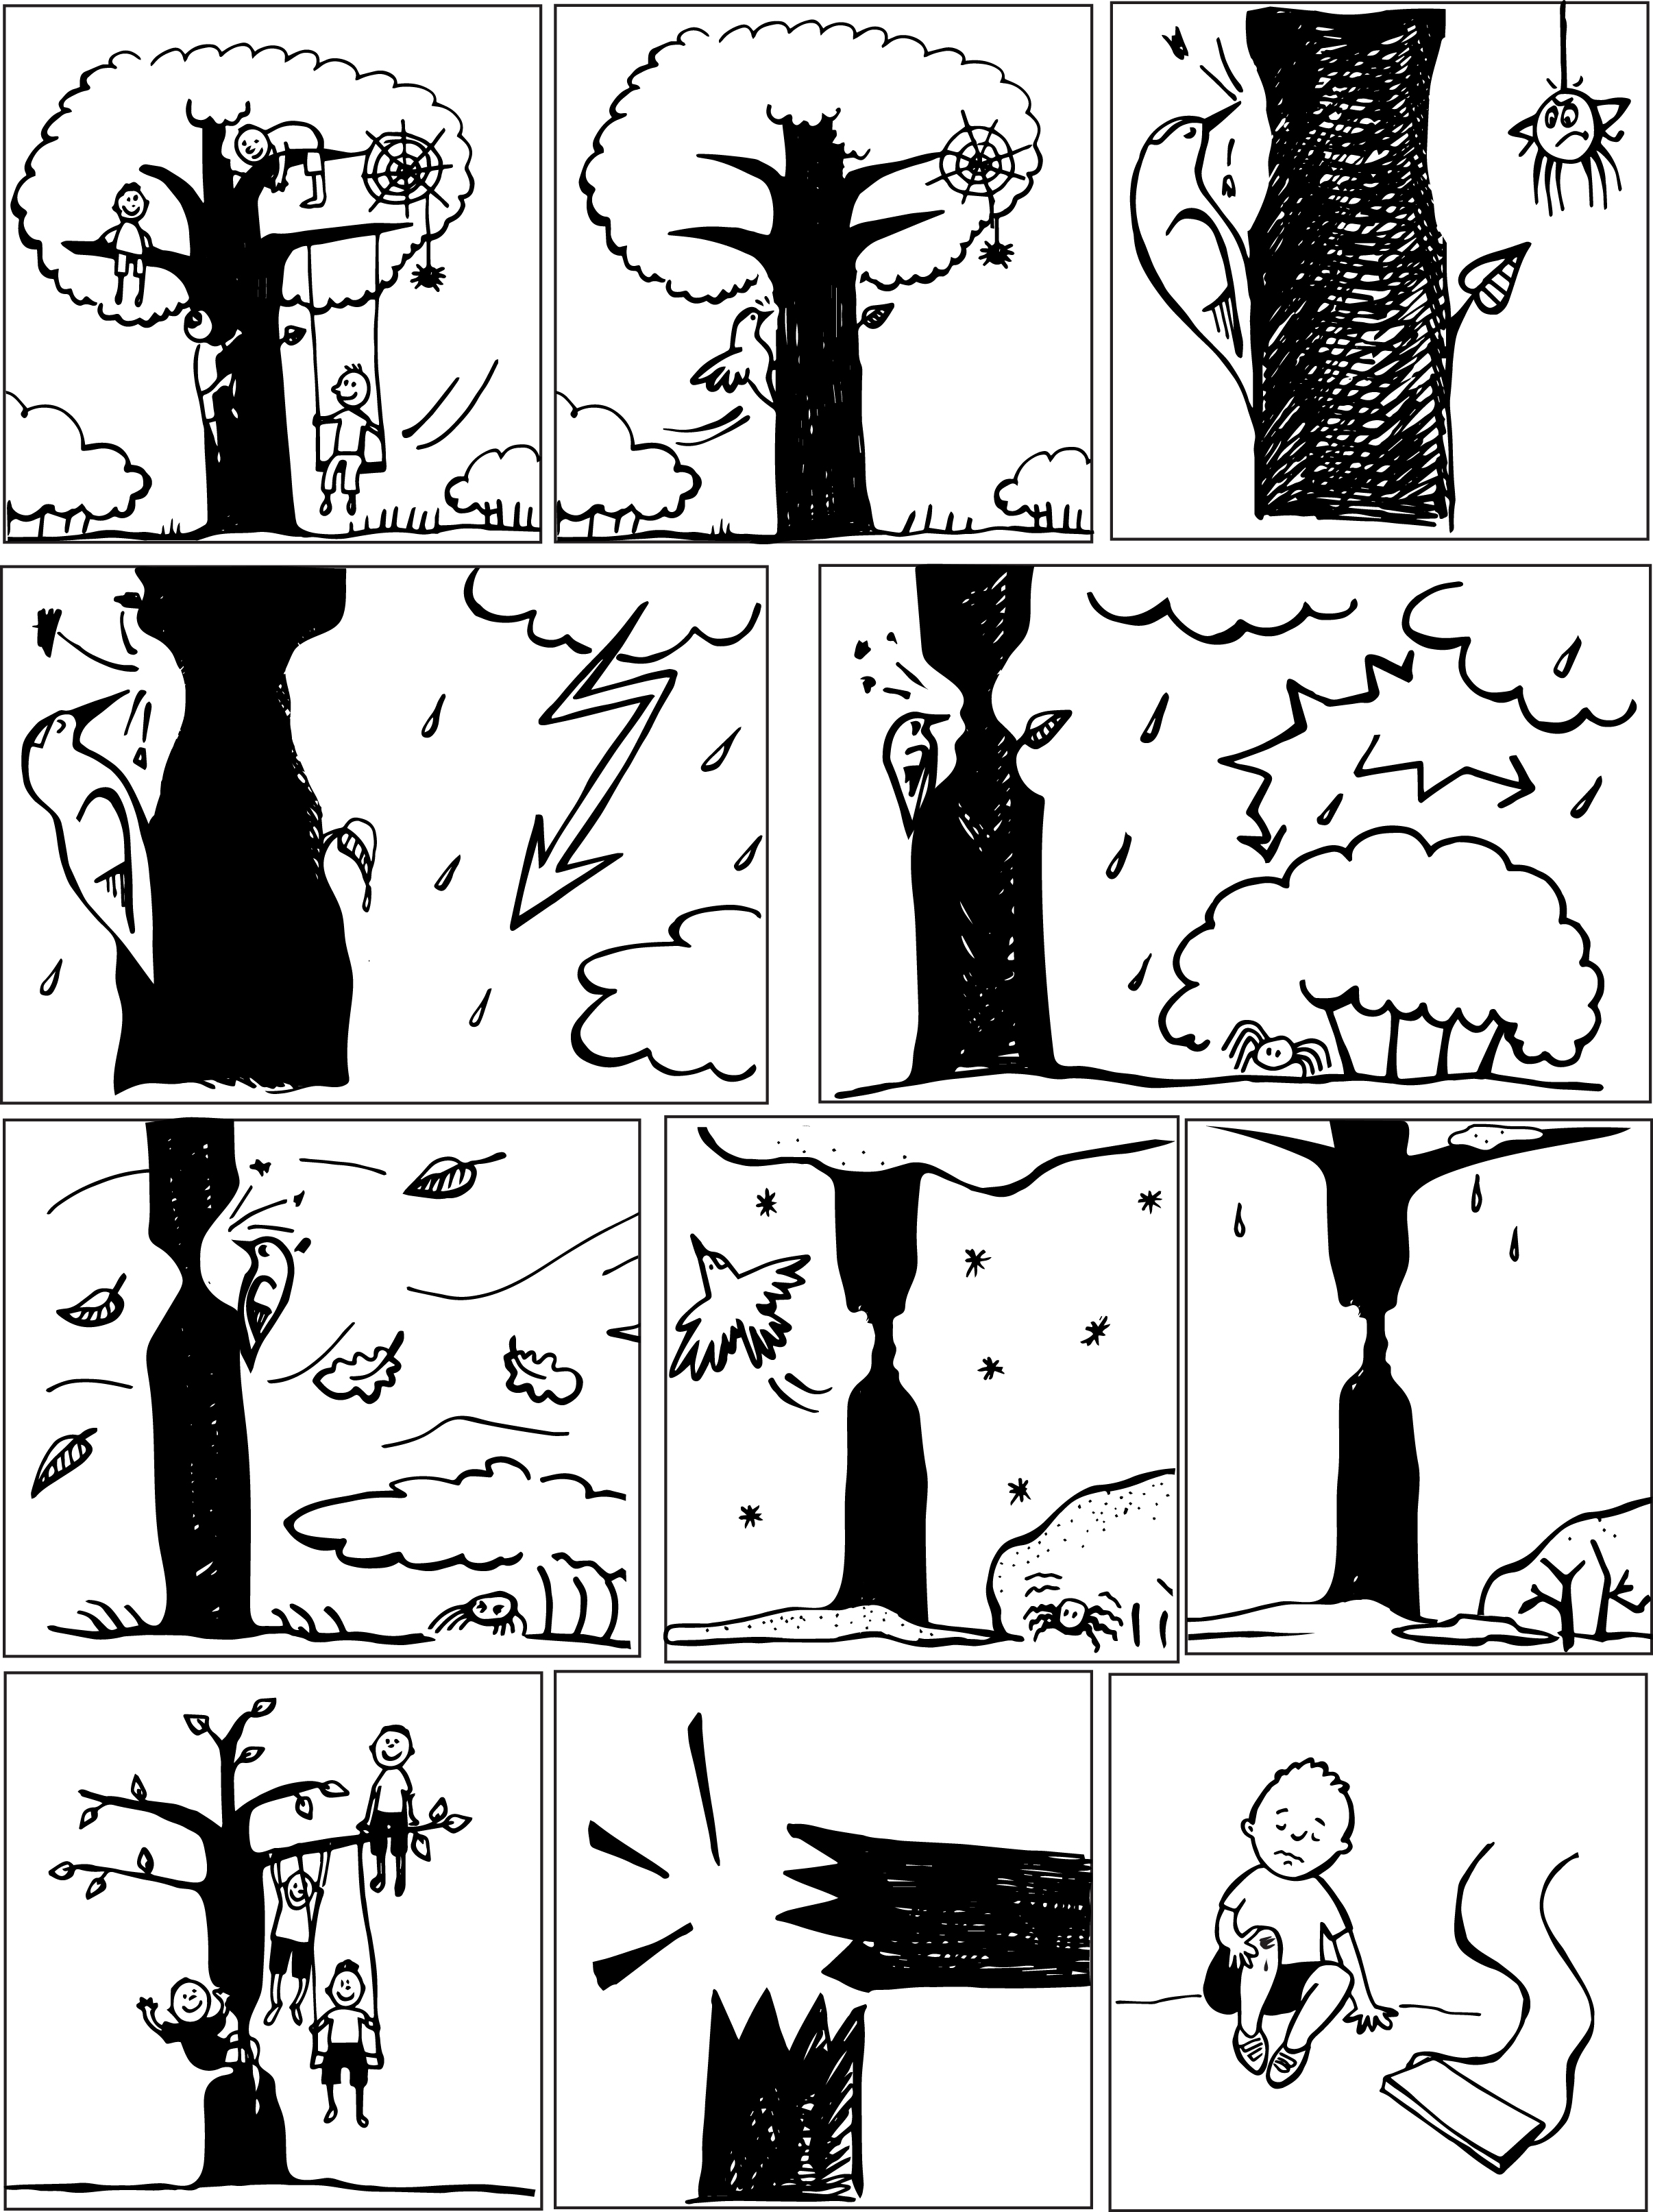
\includegraphics[width=\linewidth]{pauk.jpg}\\
\pagebreak\\
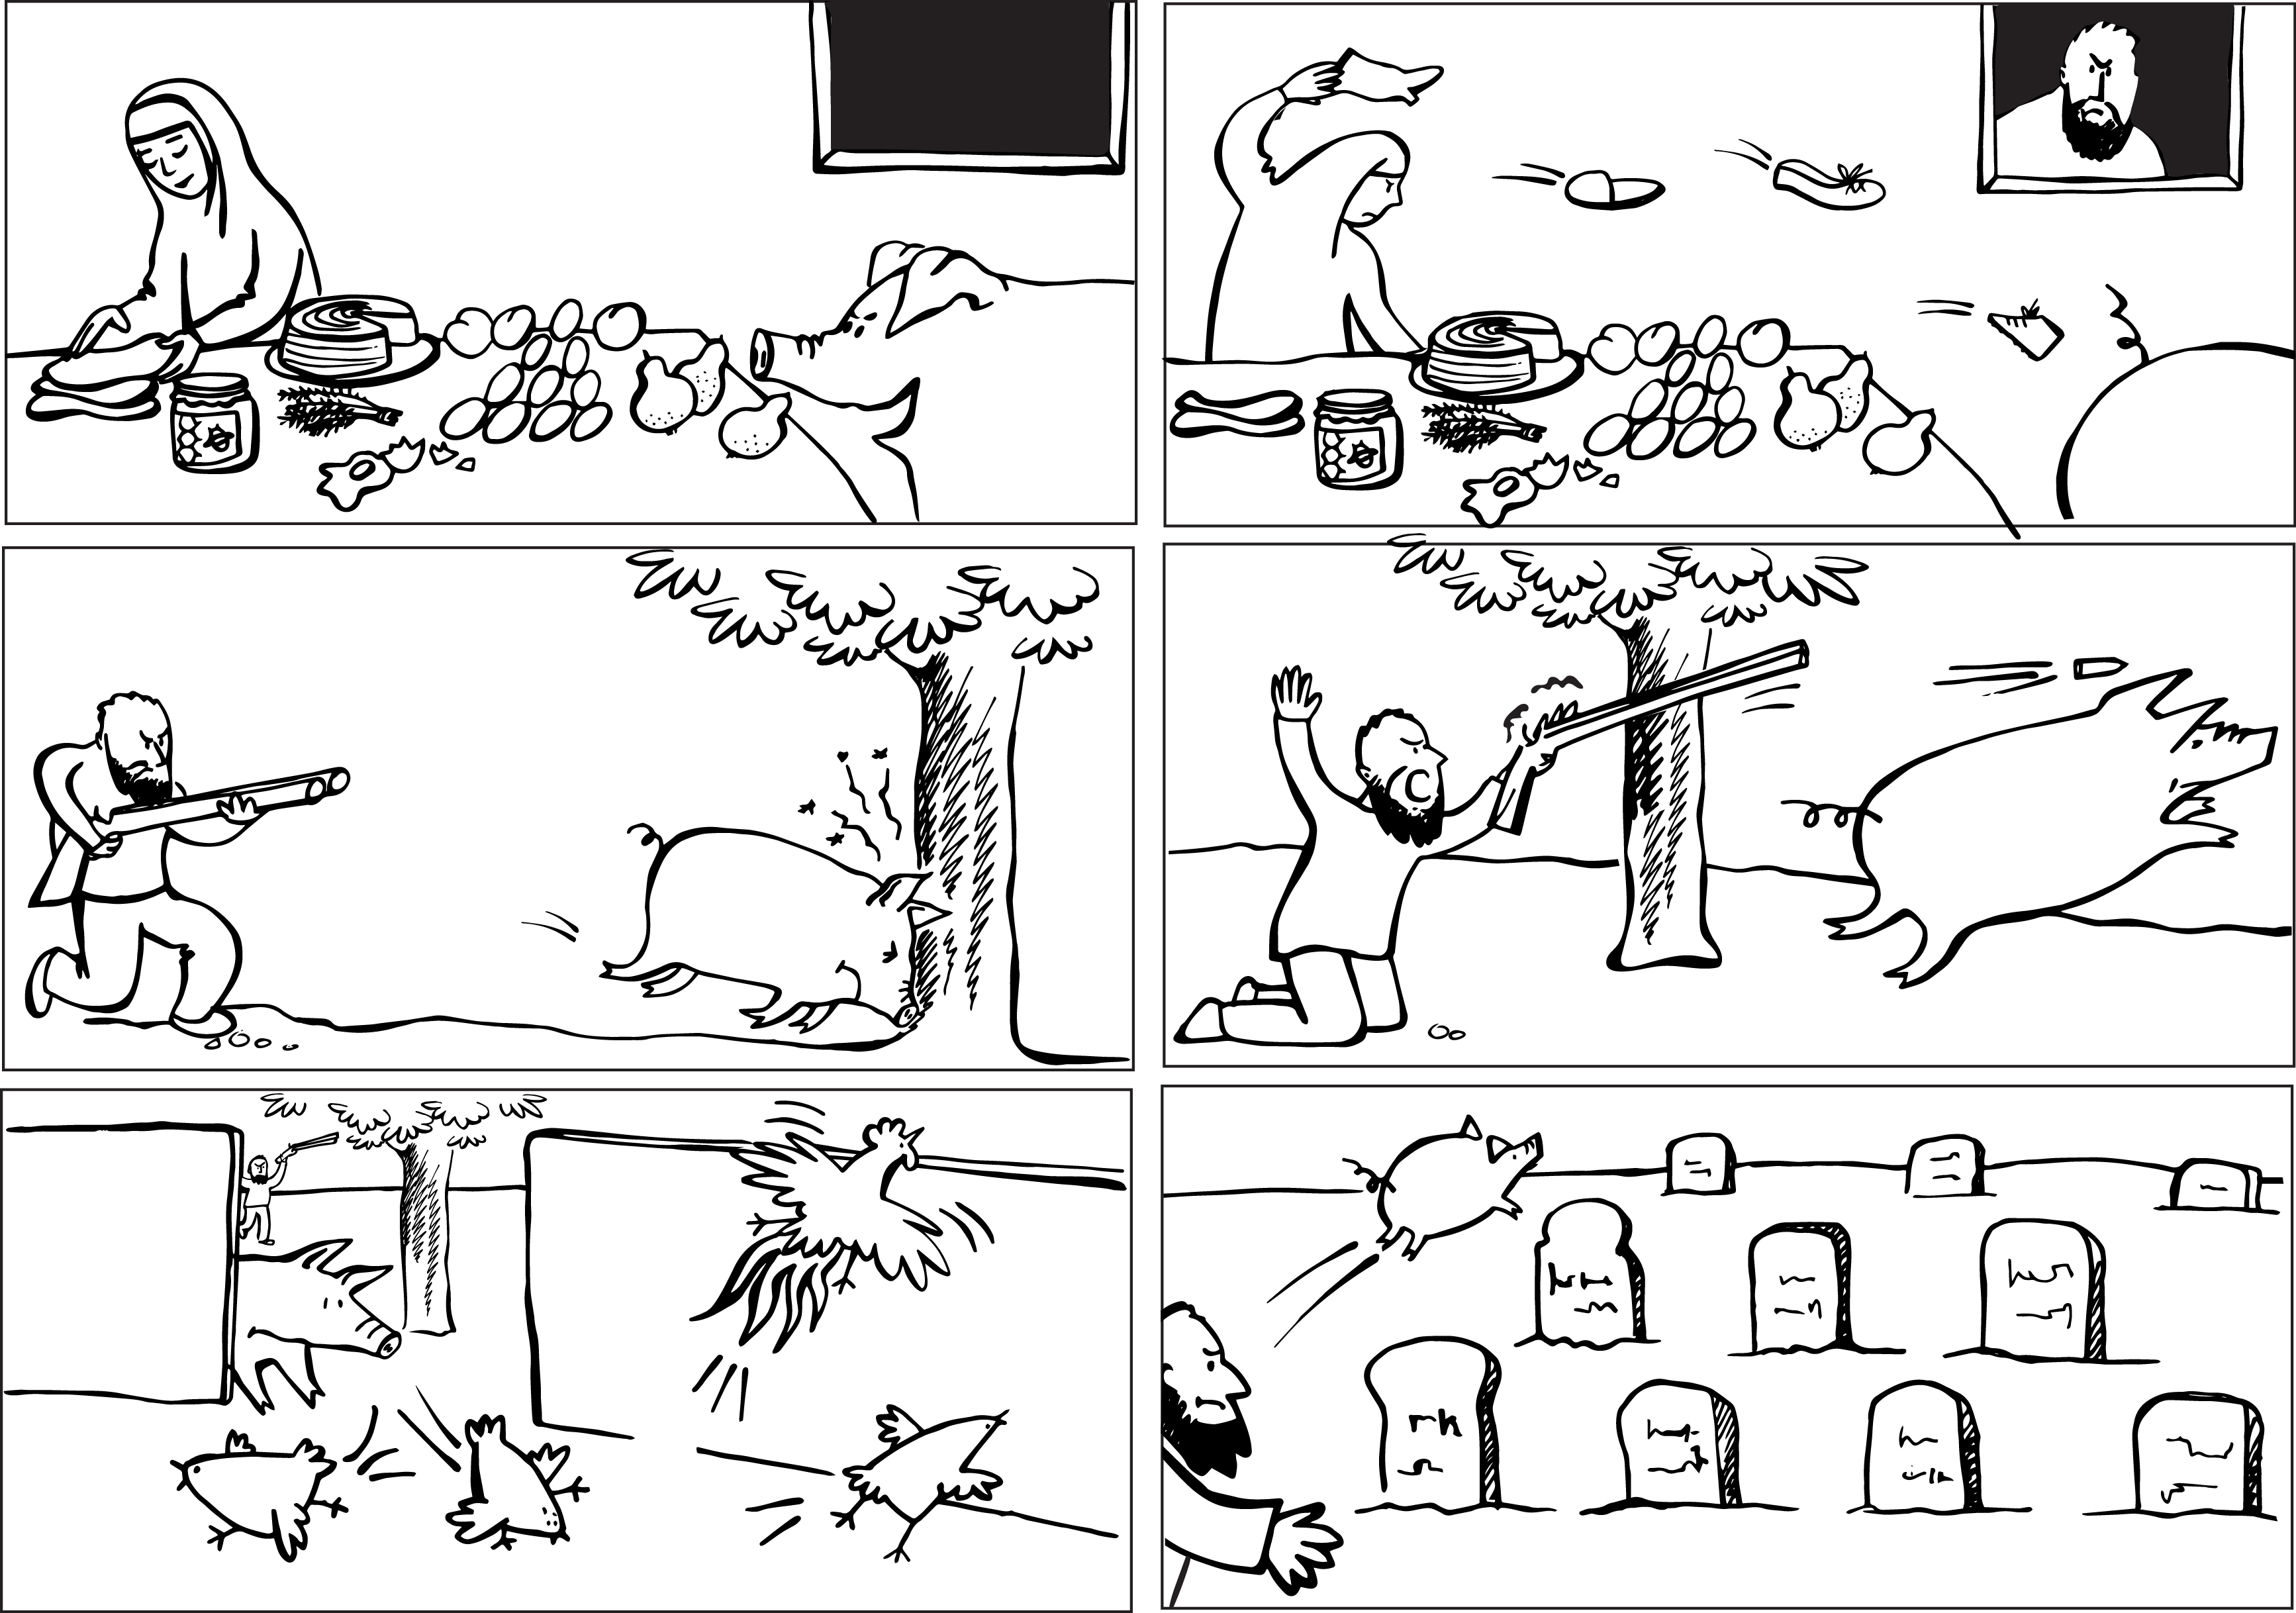
\includegraphics[width=\linewidth]{svinja.jpg}\\
\pagebreak
\subsection{Приложение 2: стихотворение Алима Кешокова} \label{text}
{~}\medskip\\
\noindent Зыхэс удз Iувыр ирецIынэ,\\
И Iэщхьэр лъагэу дэхьеяуэ\\
Хъыджэбз нэкIуплъым епщ хупцIынэ,\\
Щхьэщысщ ар Iэнлъэм зигъэзхъауэ.\medskip\\
ЕIуящIэ защIэу щIалэ куэди\\
КъетIысэкIауэ мэгушыIэ.\\
И уз а пщафIэми укIуэди,\\
Сыт къыхуапсэлъми зешыIэ.\medskip\\
ТIэкIу зигъэщхъакъэ --- псори маплъэ,\\
А щIалэр зэплъыр къыпхуэмыщIэ,\\
Хъыджэбзырщ зыщIэр псом я пIалъэ ---\\
Зигу къэплъым и Iур ирегъущIэ.\medskip\\
И щхьэцыр пщащэм ирекъуэкIыр,\\
Хьэжыгъэр нэIум къытощащэ.\\
Гу лъумытэну я гум къэкIым,\\
ЩIалэжьхэр къеплъмэ мэIущащэ.\medskip\\
Я мэлхэр шытхым щхьэдэхами,\\
Мэлыхъуэр зыкIи мыгузавэ.\\
Дэтхэнэм жьэкIэ сыт жиIами,\\
Я плырыр псалъэм щIрагъавэ.\medskip\\
Зырыз мэл хъущэу къыдахуащ,\\
АрщхьэкIэ псоми зыщ ягъэхъур.\\
А хъыджэбз пщафIэм дихьэхащ --- \\
Апхуэдэу махуэр жэщ ягъэхъур. \medskip\\
Сыт щIалэ жанхэри зезыхьэр?\\
Мэлыхъуэм я гур хьэхугъуафIэщ,\\
Хъыджыбзым ищIрэ щIакхъуэ Iыхьэ,\\
Iухуакъэ, ишхыр хъунущ мафIэ.\medskip\\
\textit{Алим КIыщокъуэ, Тхыгъэхэр, томихым щызэхуэхьэсауэ ---  Налщык: <<Эльбрус>>, 2004. --- н. 147}
\pagebreak
\subsection{Приложение 3: код в Praat (v. 5.3.16)} \label{praatscript}
\noindent Данный скрипт был написан Mietta Lennes, однако я несколько изменил его для своего удобства. Теперь он вытаскивает название всех фрагментов (в случае паузы название отсутствует), длительность, время начала фрагмента и время конца фрагмента.
\scriptsize
\begin{alltt}
# This script is distributed under the GNU General Public License.
# Copyright 17.3.2002 Mietta Lennes

form Make text file from an IntervalTier in the selected TextGrid object
	comment Which tier do you want to convert to text?
	integer Tier 1
	comment Where do you want to save the text file?
	text path /home/agricolamz/_DATA/OneDrive1/_Work/duration.txt
endform

overwrite = 0

numberOfIntervals = Get number of intervals... tier

for interval from 1 to numberOfIntervals
	start = Get starting point... tier interval
	end = Get end point... tier interval
	duration = end - start
	label$ = Get label of interval... tier interval
	if fileReadable (path$) and overwrite = 0 and interval = 1
		pause There already is a text file 'path$'. Do you want to continue and overwrite it?
		overwrite = 1
		filedelete 'path$'
	endif
	textline$ = "'label$''tab$''duration''tab$''start''tab$''end''newline$'"
	fileappend 'path$' 'textline$'
endfor

echo Created a text file 'path$' for the segments and labels in tier 'tier'

# the end of the script
\end{alltt}
\normalsize
\pagebreak
\subsection{Приложение 4: код в R (v. 3.3.1)} \label{Rscript}
\noindent Данный скрипт принимает на вход данные полученные скриптом Praat, считает общую скорость речи (speach.rate) и скорость артикуляции (articulation.rate) и рисует график, отображающий изменение скорости речи во время речепроизводства.
\scriptsize
\begin{alltt}
# get file ----------------------------------------------------------------
setwd("/home/agricolamz/_DATA/OneDrive1/_Work/_Handouts/2016 II Adyghe expedition/test from mashe")
df <- read.csv("duration.txt", sep = "\t", header = F)
names(df) <- c("number.of.syllables",
               "duration",
               "start",
               "end")
df <- df[-1,]
df[is.na(df$number.of.syllables),]$number.of.syllables <- 0

# segments without pauses
dfnp <- df[df$number.of.syllables > 0,]
dfnp <- dfnp[complete.cases(dfnp),]

# speach rate and articulation rate (syllables / min) ---------------------
speach.rate <- sum(df$number.of.syllables,na.rm = T)/df$end[nrow(df)]*60
articulation.rate <- sum(dfnp$number.of.syllables, na.rm = T)/dfnp$end[nrow(dfnp)]*60

# moving average ----------------------------------------------------------
width <- 15 # width of the moving average

library(zoo)
mmean <- rollapply(df$number.of.syllables, width, FUN = mean)
mduration <- rollapply(df$duration, width, FUN = mean)

dfmmean <- data.frame(x = df$end[1:length(mmean)],
                      res = mmean/mduration)

library(ggplot2)
ggplot(df, aes(end, number.of.syllables))+
  geom_point()+
  geom_line(data = dfmmean, aes(x, res))+
  theme_bw()+
  ylab("количество слогов")+
  xlab("время (c)")

# the end of the script
\end{alltt}
\normalsize
\end{document}